\lab{Algorithms}{Introduction to Wavelets}{Intro to Wavelets}

\objective{This lab explains the basic ideas of Wavelet Analysis
using the Haar wavelet as a prototypical example then presents applications of the Discrete Wavelet Transform in
image denoising and compression.}

Recall that in the context of Fourier analysis, one seeks to represent a
function in the frequency domain, and this is accomplished via the Fourier
transform. The Fourier transform allows us to analyze and process functions
in many useful ways, as you have seen in previous labs. There are, however,
drawbacks to this approach. For example, although a function's Fourier
transform gives us complete information on its frequency spectrum, time
information is lost. We can know which frequencies are the
most prevalent, but not when they occur. This is due in part to the fact that
the sinusoidal function $f(x) = e^{2\pi ix}$ -- on which the Fourier transform
is based -- has infinite support. Its nature is essentially \emph{non-local},
and so the Fourier transform fails to provide local information in both the
time and frequency domains. This brings us to the following question: are
there types of transforms that avoid the shortcomings mentioned above? The
answer is an emphatic yes. Enter Wavelet analysis.

\subsection*{The Haar Wavelet}

As noted earlier, the Fourier transform is based on the complex exponential
function. Let us alter the situation and consider instead the following
function, known as the \emph{Haar wavelet}:
\begin{equation*}
\psi(x) =
 \begin{cases}
  1 & \text{if } 0 \leq x < \frac{1}{2} \\
  -1 & \text{if } \frac{1}{2} \leq x < 1 \\
  0 & \text{otherwise.}
 \end{cases}
\end{equation*}

% It might be nice to plot this function and include the image in the lab.

Along with this wavelet, we introduce the associated \emph{scaling function}:
\begin{equation*}
\phi(x) =
 \begin{cases}
 1 & \text{if } 0 \leq x < 1 \\
 0 & \text{otherwise.}
 \end{cases}
\end{equation*}

From the wavelet and scaling function, we can generate two countable families
of dyadic dilates and translates given by
\begin{equation*}
\psi_{m,k}(x) = \psi(2^mx - k)
\end{equation*}
\begin{equation*}
\phi_{m,k}(x) = \phi(2^mx - k),
\end{equation*}
where $m,k \in \mathbb{Z}$.

Let us focus for the moment on that second family of functions, $\{\phi_{m,k}\}$.
If we fix $m$ and let $k$ vary over the integers, we have a countable collection of
simple functions. The support of a typical function $\phi_{m,k}$ is the interval
$[k2^{-m}, (k+1)2^{-m}]$, and for any $m \in \mathbb{Z}$ we have
\begin{equation*}
\mathbb{R} = \displaystyle\biguplus_k\,[k2^{-m}, (k+1)2^{-m}],
\end{equation*}
where $\uplus$ denotes a union over disjoint sets. Thus, the supports can be viewed as
a discretization of the real line, and we can use this collection of simple functions
to approximate any $f \in L^2(\mathbb{R})$ in the following sense:
\begin{equation*}
f(x) \approx f_m(x) := \displaystyle\sum_{k \in \mathbb{Z}}\alpha_{m,k}\phi_{m,k}(x),
\end{equation*}
where
\begin{equation*}
\alpha_{m,k} := 2^m \displaystyle \int_{k2^{-m}}^{(k+1)2^{-m}}f(x) dx
\end{equation*}
($\alpha_{m,k}$ is simply the average value of $f$ on $[k2^{-m},(k+1)2^{-m}]$). As you
would probably expect, the point-wise error between $f$ and its approximation $f_m$
(called a \emph{frame}) goes to zero as $m \to \infty$.

These frames are not quite good enough, however. Each coefficient $\alpha_{m,k}$
certainly captures local information about $f$ -- namely its average value on
a certain interval -- but it fails to tell us anything about how $f$ changes
on that interval. We need more information than is provided by $f_m$ in order
to know about discontinuities or high-frequency oscillations of $f$. To this end,
we now consider the wavelet function $\psi$.
Notice that the Haar wavelet is oscillatory in nature, and is thus better suited
to capture local information on how a function changes at a given point. For
any given $m$, we define a function $d_m$, called a \emph{detail}, as follows:
\begin{equation*}
d_m(x) := \displaystyle\sum_{k \in \mathbb{Z}}\beta_{m,k}\psi_{m,k}(x),
\end{equation*}
where
\begin{equation*}
\beta_{m,k} := 2^m \displaystyle \int_{-\infty}^{\infty}f(x) \psi_{m,k}(x) dx.
\end{equation*}
Each coefficient $\beta_{m,k}$ gives information about how $f$ changes on the
the interval $[k2^{-m}, (k+1)2^{-m}]$, and larger coefficients correspond
to larger spikes of width $2^{-m}$. Thus, as $m$ increases, the
detail function $d_m$ gives information about the higher-frequency oscillations
of the function. The details and approximation frames interact in the following way:
\begin{equation*}
f_{m+1} = f_m + d_m.
\end{equation*}
As a result of this fortuitous relationship, one can prove the decomposition
\begin{equation*}
L^2(R) = V_0 \oplus W_0 \oplus W_1 \oplus \cdots,
\end{equation*}
where $V_j := \text{span}\{\phi_{j,k}\}_{k \in \mathbb{Z}}$ and
$W_j := \text{span}\{\psi_{j,k}\}_{k \in \mathbb{Z}}$. This fact justifies
our hope to approximate and analyze functions using wavelets.
\begin{figure}[t]
\minipage{0.32\textwidth}
    \includegraphics[width=\linewidth]{sinecurve}
    \caption{$f(x) = \sin (x)$}
\endminipage\hfill
\minipage{0.32\textwidth}
    \includegraphics[width=\linewidth]{discreteSineCurve.pdf}
    \caption{$f_4$}
\endminipage\hfill
\minipage{0.32\textwidth}
    \includegraphics[width=\linewidth]{sineCurveDetail}
    \caption{$d_4$}
\endminipage
\end{figure}
\begin{problem}
Calculate and plot the approximation frames for $f(x) = \sin(x)$ on the interval $[0,2\pi]$
for $m = 4, 6, 8$. Note that because we are working on a finite interval,
we only need to calculate certain coefficients $\alpha_{m,k}$. In
particular, we only need the coefficients for $k = 0$ up to the first integer
$n$ such that $(n+1)2^{-m} > 2 \pi$ (why?). Furthermore, to plot the frame,
all we need is an array containing the relevant coefficients. Then simply plot
the coefficients against \li{linspace} with appropriate arguments
and set \li{drawstyle='steps'} in the \li{plt.plot} function.
\end{problem}

\begin{problem}
Now calculate the details for $f(x) = \sin(x)$ on the same interval and for the
same $m$ values given above. Use previous results to compute the coefficients
for $f_5$, $f_7$, and $f_9$ and plot them.
\end{problem}

\subsection*{The Discrete Wavelet Transform}

What purpose do these details and approximation frames serve? According to the
properties discussed above, we can approximate $L^2$ functions as follows:
\begin{align*}
f \approx f_{J+1} &= f_J + d_J \\
&= f_{J-1} + d_{J-1} + d_J \\
& \ldots\\
&= f_{I} + d_{I} + d_{I+1} + \cdots + d_J,
\end{align*}
where $1 \leq I \leq J$. If $f$ has compact support (as in the case of a finite-time signal,
for example), only finitely many of the coefficients in the frame and the details are
nonzero, thus enabling us to represent $f$ to a reasonable degree of accuracy in a very
efficient manner. The calculation of these detail coefficients is called the \emph{discrete
wavelet transform}. In the context of signals processing, one can imagine calculating these
coefficients, transmitting them, and then reproducing the approximated signal on the
receiving end. Furthermore, the coefficients of the details reflect the local properties
of the original function $f$ at the particular level of detail and resolution! This means
that we can discard many of the coefficients if we are only interested in reproducing a certain
part of the signal, or in recovering the entire signal to only a limited resolution. We can
also study just those frequencies of the signal that fall within a certain range (called a
sub-band) by examining the detail coefficients at a particular level. These
properties make the discrete wavelet transform an attractive alternative to the Fourier
transform in many applications. See Figure \ref{fig:dwt1D} for an example of the discrete Wavelet transform.

\begin{figure}
\centering
\includegraphics[width = 0.5\textwidth]{dwt1D}
\caption{A level 4 wavelet decomposition of a signal. The top panel is the original signal,
the next panel down is the approximation frame, and the remaining panels are the detail coefficients.
Notice how the approximation frame resembles a smoothed version of the original signal, while the 
details capture the high-frequency oscillations and noise.}
\label{fig:dwt1D}
\end{figure}

In practice, we are often interested in analyzing discrete signals with compact support (that is,
finite-time signals that we have sampled at a finite number of points). If wavelet analysis is
to be of any use, we first need an efficient way to calculate the discrete wavelet transform.
The process described in the first section, while intuitive and illustrative of the mathematical
principles
behind wavelet analysis, is not the best approach to calculating the wavelet coefficients. It
turns out that the discrete wavelet transform can be implemented as an iterated low-pass/high-pass
filter bank, one iteration of which is shown graphically in the figure. We present the
algorithm without getting into the details of why it works.
\begin{figure}[H]
\centering
\includegraphics[width = 0.5\textwidth]{dwt1}
\caption{The one-dimensional discrete wavelet transform.}
\end{figure}
The input, $A_j$, represents the level-$j$ approximation frame, and we initialize $A_0$ to
simply be the original signal. Lo and Hi are the low-pass and high-pass filters, respectively.
(By \emph{filter} we mean a vector that serves the purpose of extracting or suppressing a
particular feature of the signal. The Lo and Hi filters are obtained from the wavelet at hand;
for the Haar wavelet, Lo $= (\sqrt{2}^{-1}, \sqrt{2}^{-1})$ and Hi $= (-\sqrt{2}^{-1}, \sqrt{2}
^{-1})$.) The box means convolve the input with the filter, and the circle means downsample by
a factor of two, i.e. remove either the even or odd-indexed entries of the input. The outputs,
$A_{j+1}$ and $D_{j+1}$, are the level-$(j+1)$ approximation frame and detail coefficients,
respectively. Note that the length of the input array is twice that of the output arrays. The
detail coefficients $D_{j+1}$ are stored, and $A_{j+1}$ is then fed back into the loop. Continue
this process until the length of the output is less than the length of the filters, and
return all of the stored detail coefficients as well as the final approximation frame.
\begin{problem}
Write a function that calculates the discrete wavelet transform as described above.
The inputs should be three one-dimensional NumPy arrays (the signal, low-pass filter, and
high-pass filter). The output should be a list of one-dimensional NumPy arrays in the
following form: $[A_n, D_n, \ldots, D_1]$. (Note: for the convolution, you may use
the \li{fftconvolve} function from the \li{scipy.signal} package using the default
\li{mode = 'full'} parameter, but note that the output array is one entry too large, and so
you need to omit the first entry. For downsampling, only keep the even-indexed entries.)
\end{problem}
We also need to know how to reconstruct the signal from the detail coefficients and
approximation frame. Fortunately, the algorithm described above is entirely reversible,
albeit with slightly different filters:
$$\text{Lo} = (\sqrt{2}^{-1}, \sqrt{2}^{-1})$$ and
$$\text{Hi} = (\sqrt{2}^{-1}, -\sqrt{2}^{-1}).$$
Given $A_{j+1}$ and $D_{j+1}$, simply upsample both arrays (by inserting a zero after
each entry of the original array), convolve the results
with the Lo and Hi filters, respectively (this time omit the \emph{last} entry of the
result), and add the outputs to obtain $A_j$. Continue the
process until you recover $A_0$, the original signal.
\begin{problem}
Write a function that calculates the inverse wavelet transform as described above.
The inputs should be a list of arrays (of the same form as the output of your discrete
wavelet transform function), the low-pass filter, and the high-pass filter. The output
should be a single array, the recovered signal. In order to check your work, compute
the discrete wavelet transform of a random array of length 64, then compute the inverse
transform, and compare the original signal with the recovered signal. The difference
should be very small.
\end{problem}

\subsection*{The two-dimensional Discrete Wavelet Transform}
Our discussion so far has focused on one-dimensional
discrete signals, but it is not difficult to extend the same ideas into the
realm of two-dimensional arrays. As you know, a digital image can be represented
as a matrix of pixel values (for simplicity we will consider grayscale images of
size $2^n \times 2^n$). We can perform the wavelet decomposition of
an image in much that same way as with one-dimensional signals. We once again
calculate detail and approximation coefficients using an iterative filter
bank, but now we generate four arrays of coefficients at each iteration as opposed to
just two. In essence, we perform the one-dimensional wavelet transform first on each
row, and then on each column of the matrix. Notice the similarity with our approach
to extending the one-dimensional Fourier transform to two-dimensional images. See
Figure \ref{fig:dwt2D} of an example of the two-dimensional Wavelet transform applied
to an image.

\begin{figure}
    \includegraphics[width=0.8\textwidth]{dwt2D.pdf}
    \caption{The level 2 wavelet coefficients of the Lena image. The upper left quadrant 
    is the approximation frame, and the other quadrants are the details. Notice how the 
    details highlight the parts of the image with high-frequency textures and borders.}
    \label{fig:dwt2D}
\end{figure}

The algorithm goes as follows.
Given an input matrix of size $2^n \times 2^n$, first operate on the rows as you would
in the one-dimensional Wavelet transform (i.e. convolve each row with the filters, then
downsample).
We then have two matrices of size $2^n \times 2^{n-1}$,
since each row has been downsampled by a factor of 2. Then for each of these two
intermediate matrices, operate on each column, yielding a total of four matrices of
size $2^{n-1} \times 2^{n-1}$. Figure \ref{fig:2dwt}
gives a graphical depiction of one iteration of the algorithm.

\begin{figure}[t]
    \includegraphics[width=0.8\textwidth]{2dwt.jpg}
    \caption{The 2-dimensional discrete wavelet transform.}
    \label{fig:2dwt}
\end{figure}


We initialize $LL_0$ to be the
original image matrix, and we terminate once the length of the rows or columns
is less than the length of the filters. We end up with a list of wavelet
coefficients, starting with the final approximation frame $LL_n$ followed by
collections of detail coefficients $(LH_n,HL_n,HH_n)$, $(LH_{n-1},HL_{n-1},HH_{n-1})$,
$\ldots$, $(LH_1,HL_1,HH_1)$. Note that at each iteration we operate first on the
rows (convolve with the filter, then downsample), and the we operate on the columns
of the resulting matrices (\emph{not} the original matrix). The size of the output
matrices have been reduced by a factor of two in both dimensions. As with the
one-dimensional algorithm, to reconstruct the image from the coefficients, we simply
reverse the process by upsampling, convolving, and adding (first the columns, then
the rows). We provide sample code for one iteration of the transform and the inverse.

\begin{lstlisting}
import numpy as np
from scipy.signal import fftconvolve

# given the current approximation frame image, and the filters lo_d and hi_d
# initialize empty arrays
temp = np.zeros([image.shape[0], image.shape[1]/2])
LL = np.zeros([image.shape[0]/2, image.shape[1]/2])
LH = np.zeros([image.shape[0]/2, image.shape[1]/2])
HL = np.zeros([image.shape[0]/2, image.shape[1]/2])
HH = np.zeros([image.shape[0]/2, image.shape[1]/2])

# low-pass filtering along the rows
for i in xrange(image.shape[0]):
	temp[i] = fftconvolve(image[i], lo_d, mode='full')[1::2]

# low and hi-pass filtering along the columns
for i in xrange(image.shape[1]/2):
	LL[:,i] = fftconvolve(temp[:,i],lo_d,mode='full')[1::2]
    LH[:,i] = fftconvolve(temp[:,i],hi_d,mode='full')[1::2]

# hi-pass filtering along the rows
for i in xrange(image.shape[0]):
	temp[i] = fftconvolve(image[i], hi_d, mode='full')[1::2]

# low and hi-pass filtering along the columns
for i in xrange(image.shape[1]/2):
	HL[:,i] = fftconvolve(temp[:,i],lo_d,mode='full')[1::2]
    HH[:,i] = fftconvolve(temp[:,i],hi_d,mode='full')[1::2]
\end{lstlisting}
At this point, the variables \li{LL, LH, HL, HH} contain the current level of wavelet coefficients.
You would then store \li{(LH, HL, HH)} in a list, and feed \li{LL} back into the same
block of code (with \li{LL} replacing \li{image}) to obtain the next level of coefficients.

Now, given a current level of wavelet coefficients, here is the code to recover the previous
approximation frame, which is the crucial step in the inverse transform.
\begin{lstlisting}
# given current coefficients LL, LH, HL, HH
# initialize temporary arrays
n = LL.shape[0]
temp1 = np.zeros([2*n,n])
temp2 = np.zeros([2*n,n])
up1 = np.zeros(2*n)
up2 = np.zeros(2*n)

# upsample and filter the columns of the coefficient arrays
for i in xrange(n):
	up1[1::2] = HH[:,i]
	up2[1::2] = HL[:,i]
	temp1[:,i] = fftconvolve(up1, hi_r)[1:] + fftconvolve(up2, lo_r)[1:]
	up1[1::2] = LH[:,i]
	up2[1::2] = LL[:,i]		
	temp2[:,i] = fftconvolve(up1, hi_r)[1:] + fftconvolve(up2, lo_r)[1:]

# upsample and filter the rows, then add results together
result = sp.zeros([2*n,2*n])
for i in xrange(2*n):
	up1[1::2] = temp1[i]
	up2[1::2] = temp2[i]
	result[i] = fftconvolve(up1, hi_r)[1:] + fftconvolve(up2, lo_r)[1:]
\end{lstlisting}

\begin{problem}
Build off of the sample code to fully implement the two-dimensional discrete
wavelet transform as described above.
As before, the input to your function should consist of
three arrays: the input image, the low-pass filter, and the high-pass filter.
You should return a list of the following form: $$[LL_n,(LH_n,HL_n,HH_n), \ldots
,(LH_1,HL_1,HH_1)].$$ 

The inverse wavelet transform function should take as input a list
of that same form, as well as the reconstruction low-pass and high-pass filters,
and should return the reconstructed image.
\end{problem}

These wavelet coefficients are very useful in a variety of image processing
tasks. They allow us to analyze and manipulate images in terms of both their
frequency and spatial properties, and at differing levels of resolution.
Furthermore, wavelet bases often have the remarkable ability to represent
images in a very \textit{sparse} manner -- that is, most of the image
information is captured by a small subset of the wavelet coefficients.
In the remainder of this lab, we will see how the discrete wavelet transform
plays a role in edge detection, noise removal, and compression.

\subsection*{More Wavelets}
Up to this point, the only wavelet that we have considered is the Haar wavelet,
which is the simplest and historically first example. Wavelet analysis is a broad
field, however, and there are myriad other wavelets that have been studied and
applied. Your implementation of the discrete wavelet transform is quite general,
and you will find that different types of signals or functions call for different
wavelets. We will not go into detail here, but be aware that there is a large
selection of wavelets out there.

\begin{figure}[H]
\minipage{0.49\textwidth}
    \includegraphics[width=\linewidth]{mexicanHat}
    \caption{The Mexican Hat Wavelet}
\endminipage\hfill
\minipage{0.49\textwidth}
    \includegraphics[width=\linewidth]{db5_3}
    \caption{The Cohen-Daubechies-Feauveau 5/3 Wavelet}
\endminipage
\end{figure}

\section*{The PyWavelets Module}
PyWavelets is a Python library for Wavelet Analysis. It provides convenient and
efficient methods to calculate the one and two-dimensional discrete Wavelet
transform, as well as much more. Assuming that the package has been installed on
your machine, type the following to get started:
\begin{lstlisting}
>>> import pywt
\end{lstlisting}
Performing the basic discrete Wavelet transform is very simple.
Below, we compute the one-dimensional transform for a sinusoidal signal.
\begin{lstlisting}
>>> import numpy as np
>>> f = np.sin(np.linspace(0,8*np.pi, 256))
>>> fw = pywt.wavedec(f, 'haar')
\end{lstlisting}
The variable \li{fw} is now a list of arrays, starting with the final approximation
frame, followed by the various levels of detail coefficients, just like the output
of the wavelet transform function that you coded in the previous lab.
Plot the level 2 detail and verify that it resembles a blocky sinusoid.
\begin{lstlisting}
>>> from matplotlib import pyplot as plt
>>> plt.plot(fw[-2], linestyle='steps')
>>> plt.show()
\end{lstlisting}
We can give alter the arguments to the \li{wavedec} function to use different
wavelets or obtain different levels of the wavelet transform. The second
positional argument, as you will notice, is a string that gives the name of the
wavelet to be used. We first used the Haar wavelet, with which you are already
familiar. PyWavelets supports a number of different Wavelets, however, which you can
list by executing the following code:
\begin{lstlisting}
>>> # list the available Wavelet families
>>> print pywt.families()
['haar', 'db', 'sym', 'coif', 'bior', 'rbio', 'dmey']
>>> # list the available wavelets in the coif family
>>> print pywt.wavelist('coif')
['coif1', 'coif2', 'coif3', 'coif4', 'coif5']
\end{lstlisting}
We can also include optional arguments \li{mode} and \li{level} when calling the
\li{wavedec} function. Using these arguments, you can adjust the mode for dealing
with border distortion and the level of the Wavelet decomposition, respectively.

\begin{figure}[t]
    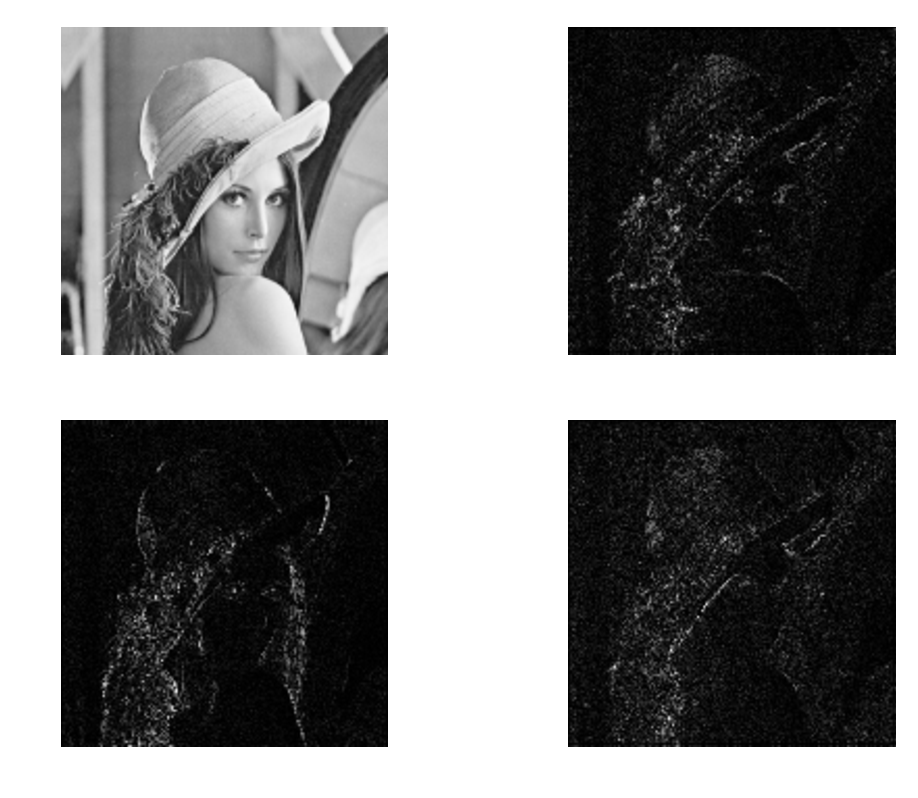
\includegraphics[width=\linewidth]{dwt2.pdf}
    \caption{Level 1 Wavelet decomposition of the Lena image.
    The upper left is the approximation frame, and the remaining
    plots are the detail coefficients.}
    \label{fig:dwt2}
\end{figure}

Now we illustrate how to perform a two-dimensional Wavelet transform using
PyWavelets. We will work with the traditional Lena image, performing a
two level wavelet transform using the Daubechies 4 Wavelet.
\begin{lstlisting}
>>> import scipy.misc
>>> lena = scipy.misc.lena()
>>> lw = pywt.wavedec2(lena, 'db4', level=2)
\end{lstlisting}
The variable \li{lw} is a list of tuples of arrays. The first entry of the list is
simply the level 2 approximation frame. The second entry of the list is a tuple of
the level 2 detail coefficients $LH$, $HL$, and $HH$ (in that order). The remaining
entries of the list are tuples containing the lower level detail coefficients.
Thus, to plot the level 1 $HL$ detail coefficients, we can execute the following code:
\begin{lstlisting}
>>> HL1 = lw[-1][1]
>>> plt.imshow(np.abs(HL1), cmap=plt.cm.Greys_r, interpolation='none')
>>> plt.show()
\end{lstlisting}
The output of this code should be a plot resembling the lower left plot given in Figure
\ref{fig:dwt2}.

We have only introduced a couple of the basic tools available in PyWavelets. There
are of course many more functions and methods that facilitate a more comprehensive
Wavelet analysis. In the remainder of this lab, we will explore three particular 
applications of Wavelet analysis in the realm of image processing and compression.

%\section*{Edge Detection}
%It is often useful to identify the edges of objects and figures
%represented in images. The edge information can be used to classify images
%and group them with other similar images (this is part of a field called
%\textit{computer vision}), to segment the image into component parts, to
%sharpen blurry images, to filter out unnecessary details of the image,
%and so forth. Of course, our human eyes are very adept at recognizing edges,
%but enabling a computer to do the same is much more difficult. An edge can
%be thought of as a discontinuity in the image or a region of high contrast
%in either color or brightness. We can therefore leverage the high-frequency
%detail coefficients of the wavelet transform to detect the edges. Execute the
%following code:
%\begin{lstlisting}
%>>> # calculate one level of wavelet coefficients
%>>> coeffs = pywt.wavedec2(lena,'haar', level=1)
%\end{lstlisting}
%
%Note that the approximation coefficients are very close to the original
%image, while the detail coefficients are much more sparse, and roughly
%capture the edges in the image. In particular, the upper right coefficients
%emphasize the vertical edges, the lower left coefficients emphasize the
%horizontal edges, and the lower right coefficients emphasize the diagonal
%edges.
%
%\begin{problem}
%Now zero out the approximation coefficients and use your inverse DWT
%function to recreate the image. Plot its absolute value. This image is
%a fairly good representation of the edges. If we add this to the original
%image, we can increase the contrast at the edges (that is, make the dark
%side darker, and the light side lighter). Do this, and plot the original
%image side-by-side with the sharpened image. What do you notice? There
%are many image-sharpening techniques, and those based on wavelets
%are more sophisticated than what we have done here, but this gives the
%basic idea.
%\end{problem}
%the above section needs work, or maybe should be taken out completely.

\section*{Noise Removal}
Noise in an image can be defined as unwanted visual artifacts that
obscure the true image. Images can acquire noise from a variety of
sources, including the camera, transmission, and image processing
algorithms. Noise can be completely random and incoherent (as in
Figure \ref{fig:incoherent}), or it can be coherent and display
visual patterns (Figure \ref{fig:coherent}). In this section, we will
focus on reducing a particular type of random noise in images, called
\textit{Gaussian white noise}.

\begin{figure}[t]
\minipage{0.49\textwidth}
    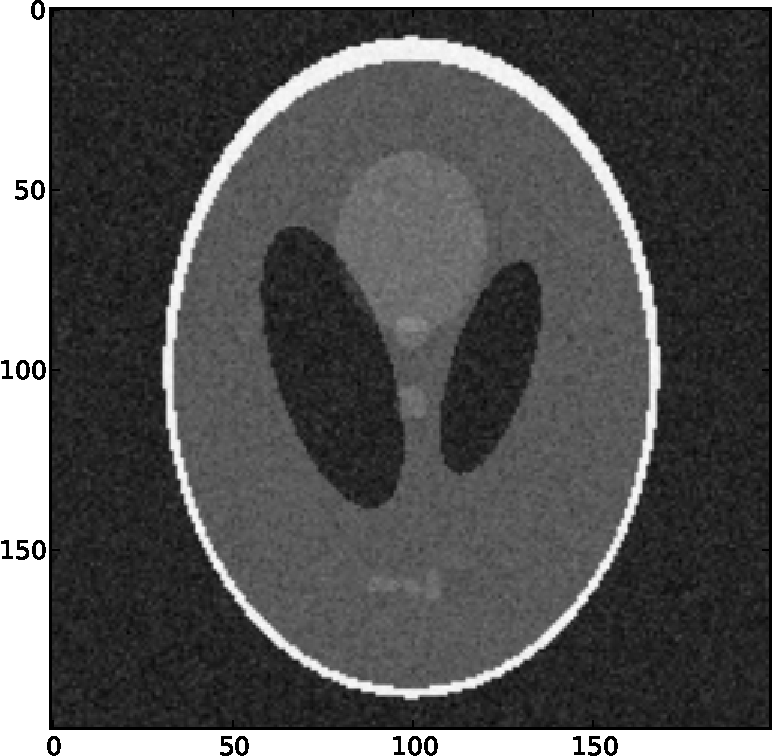
\includegraphics[width=\linewidth]{phantom_random.pdf}
    \caption{The Phantom image with incoherent noise}
    \label{fig:incoherent}
\endminipage\hfill
\minipage{0.49\textwidth}
    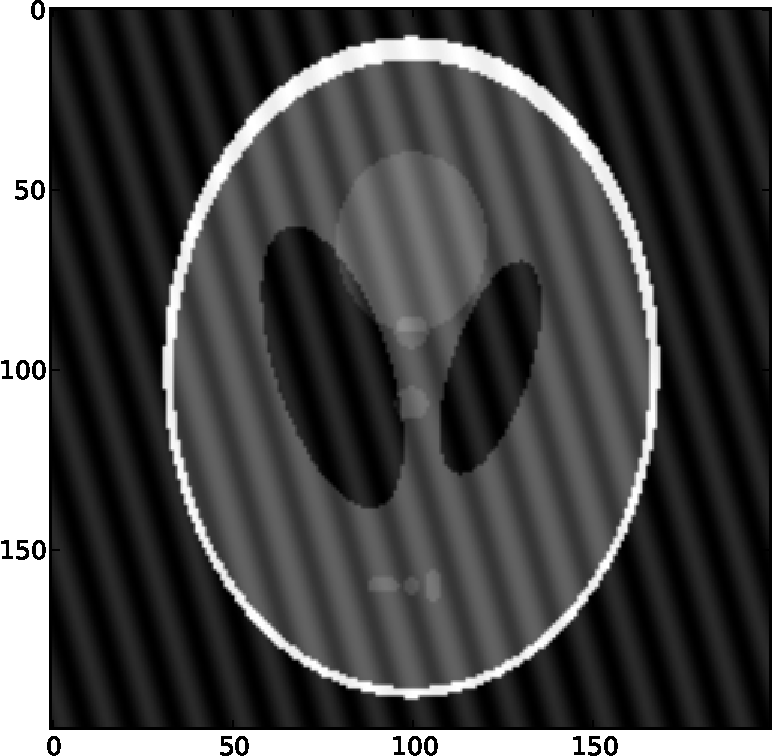
\includegraphics[width=\linewidth]{phantom_coherent.pdf}
    \caption{The Phantom image with coherent noise}
    \label{fig:coherent}
\endminipage
\end{figure}

An image that is distorted by Gaussian white noise is one in which
every pixel has been perturbed by a small amount, such that the
perturbations are normally distributed. We can easily add such noise
to an image using the \li{np.random.normal} function.

\begin{lstlisting}
>>> noisyLena = lena + np.random.normal(scale=20, size=lena.shape)
>>> plt.imshow(noisyLena, cmap=plt.cm.Greys_r)
>>> plt.show()
\end{lstlisting}

Given an image with Gaussian white noise, how do we go about reducing
the noise level? Our approach will be based on the idea of thresholding.
It turns out that images are often sparse in the wavelet basis,
particularly in the high-frequency details. The Gaussian noise, however,
is very high frequency, and thus its wavelet transform will be
concentrated in high-frequency wavelet coefficients (of magnitude
roughly proportional to the variance of the noise). We can therefore
reduce the noise while preserving the true image by shrinking the
detail coefficients via hard or soft thresholding.

Given a positive threshold value $\tau$, hard thresholding sets
every wavelet coefficient whose magnitude is less than $\tau$ to
zero, while leaving the remaining coefficients untouched. Soft
thresholding also zeros out all coefficients of magnitude less than
$\tau$, but in addition maps every other coefficient $\beta$ to
$\beta - \tau$ if $\beta > 0$ or $\beta + \tau$ if $\beta < 0$.

Implementing these simple thresholding algorithms in Python is 
straight-forward, but PyWavelets already provides this functionality.
The following code gives an example.

\begin{lstlisting}
>>> A = np.arange(-4,5).reshape(3,3)
>>> A
array([[-4, -3, -2],
       [-1,  0,  1],
       [ 2,  3,  4]])
>>> pywt.thresholding.hard(A,1.5)
array([[-4, -3, -2],
       [ 0,  0,  0],
       [ 2,  3,  4]])
>>> pywt.thresholding.soft(A,1.5)
array([[-2.5, -1.5, -0.5],
       [ 0. ,  0. ,  0. ],
       [ 0.5,  1.5,  2.5]])
\end{lstlisting}

Once the coefficients have been thresholded, we take the inverse
wavelet transform to recover the denoised image. This can be done
by calling the \li{waverec2} function, providing the list of Wavelet
coefficients as well as the name of the desired Wavelet as arguments.
The threshold value is generally a function of the variance of the noise,
and in real situations, we do not know what this variance is. In fact,
noise variance estimation in images is a research area in its own
right, but this goes beyond the scope of this lab, and so we will
assume that we already have a decent estimate of the variance.

\begin{figure}[t]
    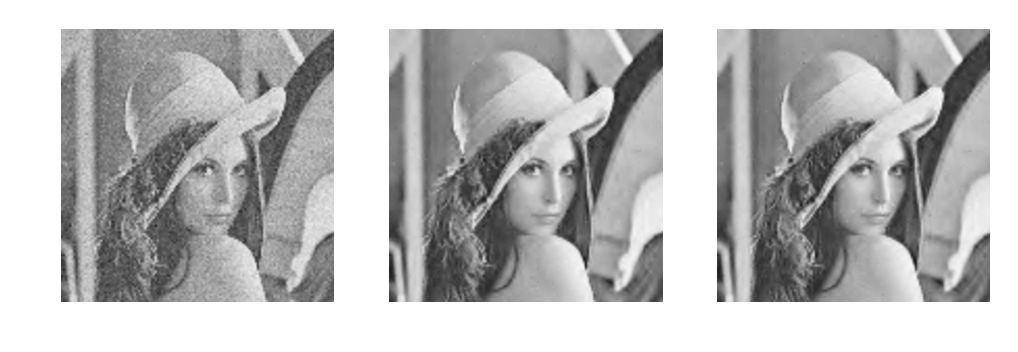
\includegraphics[width=\linewidth]{denoise.pdf}
    \caption{Noisy Lena (left), denoised using hard thresholding (center), 
    and denoised using soft thresholding (right).}
    \label{fig:denoise}
\end{figure}

\begin{problem}
Write functions that implement the hard and soft thresholding
techniques. The inputs should be a list of wavelet coefficients
in the usual form, as well as the threshold value. The output
should be the thresholded wavelet coefficients (also in
the usual form). Remember that we only want to threshold the
detail coefficients, and not the approximation coefficients.
You should therefore leave the first entry of the input
coefficient list unchanged.
\end{problem}

\begin{problem}
Create a noisy version of the Lena image by adding Gaussian
white noise of mean 0 and standard deviation $\sigma = 20$ (i.e. \li{scale=20}).
Compute four levels of the wavelet coefficients using the Daubechies 4 Wavelet, 
and input these into your
thresholding functions (with $\tau = 3\sigma$ for the hard threshold,
and $\tau = 3\sigma/2$ for the soft threshold). Reconstruct the
two denoised images, and then plot these together alongside the
noisy image. Your output should match Figure \ref{fig:denoise}.

What do you notice? How does lowering or raising the
threshold affect the reconstructed images? What happens if you use
a different Wavelet?
\end{problem}

\section*{Image Compression}
We now turn to the problem of image compression. Explicitly saving
the value of every pixel in an image can be very costly in both
storage and transmission, and numerous image compression techniques
have been developed over the years to deal with this problem.
Transform methods have long played an important role in these
techniques; the popular JPEG image compression standard is based on
the discrete cosine transform. Starting from the early 1990's, much
research has gone into compression methods using the discrete wavelet
transform, and to great success. The JPEG2000 compression standard
and the FBI Fingerprint Image database, along with other systems,
take the wavelet approach.

The general framework for compression is fairly straightforward. First,
the image to be compressed undergoes some form of preprocessing (this
can include subtracting out its mean, tiling the image, or perhaps
nothing at all). Next, the wavelet coefficients are computed using some
specially constructed wavelet (JPEG2000 uses the either the
Cohen-Daubechies-Feauveau 9/7 or 5/3 wavelet) and then \textit{quantized},
 a process that we will explain shortly. The quantized coefficients are
 then grouped in a particular way and passed through an entropy encoder
 (such as Huffman coding, run length coding, or arithmetic coding). This
 coding step comes from the realm of information theory, and we will not
 worry about it in this lab. What you have left is a compact stream of bits
 that can then be saved or transmitted much more efficiently than the
 original image. All of the above steps are invertible, allowing us to
 reconstruct the image from the bitstream.

 The step in this process that we will focus on is quantization. Put simply,
 quantization is a process whereby the coefficients are converted into
 integers. If the coefficients are floating-point numbers, then this
 process introduces some loss of precision, and we call this \textit{
 lossy compression}. In the situation where all the coefficients are already
 integers, it is possible to compress the image without any loss of precision,
 and this is called \textit{lossless compression}. Quantization can be
 performed in a variety of ways, and we will explore one particular method
 called a \emph{uniform null-zone quantizer}. Given a coefficient $x$, we assign
 to it an integer $q$ given by
\begin{equation*}
q =
 \begin{cases}
   \lceil x / \delta - t/2 \rceil, &  x \geq 0\\
   \lfloor x / \delta + t/2 \rfloor & x \leq 0
 \end{cases}
\end{equation*}
where $1 \leq t \leq 2$ and $\delta > 0$ are adjustable parameters.
The inverse process, called de-quantization, consists of recovering
the coefficient $y$ from the quantized value $q$ via the equation
\begin{equation*}
 y =
  \begin{cases}
   (q - 1/2 + t/2)\delta & q > 0\\
   (q + 1/2 - t/2)\delta & q < 0\\
   0,                    & q = 0
  \end{cases}
 \end{equation*}
What we are essentially doing is mapping all wavelet coefficients that
fall in the interval $[-\delta,\delta]$ to 0 and all wavelet coefficients
in the interval $[j\delta,(j+1)\delta]$ to $(2j+1)\delta/2$ for integers
$j \geq 1$ and $j \leq -2$. This greatly reduces the number of distinct
coefficient values (indeed, most of the coefficients are mapped to
zero), allowing us, at the cost of some precision, to store less
information. The larger we choose $\delta$, the more compression we
can achieve, albeit with a correspondingly larger loss in precision.
\begin{problem}
Write function \li{quantize} and \li{dequantize} based on the discussion above.
In both cases, the inputs should be a list of wavelet coefficients in
standard form, the $\delta$ parameter, and the $t$ parameter with default
value of 2. The functions should return the quantized list of wavelet
coefficients.

For the Lena image, calculate the complete set of wavelet coefficients and then
quantize and de-quantize the coefficients, and reconstruct the image.
Do this for a few different values of $\delta$ (with $t=2$), and observe how
the image is distorted. Try using different Wavelets. Keep in mind that there are
specially designed Wavelets used in image compression that are not available
in PyWavelets, so distortion will be greater than tolerable in real-life settings.
\end{problem}